% !Mode:: "TeX:UTF-8"
%%  本模板推荐以下方式编译:
%%     1. PDFLaTeX[推荐]
%%     2. xelatex [含中文推荐]
%%  注意:
%%  1. 文件默认的编码为 UTF-8 对于windows,请选用支持UTF-8编码的编辑器。
%%   2. 若是模板有什么问题,请及时与我们取得联系,Email:latexstudio@qq.com。
%%   3. 可以到  https://ask.latexstudio.net 提问
%%   4. 请安装 最新版本的 TeXLive 地址:
%%   http://mirrors.ctan.org/systems/texlive/Images/texlive.iso

\documentclass{apmcmthesis}

\usepackage{url}
\usepackage{float}

%%%%%%%%%%%%填写相关信息%%%%%%%%%%%%%%%%%%%%%%%%%%
\tihao{}                            %选题
\baominghao{}           %参赛编号
\begin{document}

%\pagestyle{frontmatterstyle}





\newpage
%目录
\tableofcontents


\newpage
%\pagestyle{mainmatterstyle}
\setcounter{page}{1}
\section{引言}
\subsection{问题背景及意义}
经过多年的发展,中国铁路客票发售和预订系
统已成为覆盖全国的超大型分
布式售票网络;12306 互联网售票系统是其中一个
最主要的售票渠道,自上线以来,以便捷性迅速得
到广泛认可,越来越多的旅客通过互联网购票,互
联网售票量呈大幅增长态势,售票高峰期的大量并
发请求给互联网售票系统带来的压力也屡创新高。\cite{1}

铁路客票系统是指中国铁路客运的制票系统,包括铁路客票发售和预订。铁路客票系统包括查询旅客列车时刻表、票价、列车正晚点、改签,退签,余票查询,选座,点餐,支付等众多功能。铁路客票系统流量巨大,最高日访问量\textbf{1500}亿次,高峰日平均1秒承受\textbf{170}多万次点击。
 
 因此,铁路客票系统功能众多,流量巨大,设计购票系统最基础功能和算法,并加以改进,在基础领域实现改进和突破,从而实现整体的提升,具有重要意义。


\subsection{售票信息管理系统}
本文通过c++及数据结构,实现了售票信息的界面设计与实现,售票信息管理系统包含登录注册功能,并分为\textbf{普通用户}和\textbf{后台管理员}界面,普通用户具有购票,查询,充值,查询历史订单等功能;后台管理员可以添加,修改,删除,查询售票信息。售票信息管理系统关闭时将用户信息与售票信息保存至\textbf{二进制}文件中,打开时读取用户信息和售票信息。





\section{任务实现过程}


\subsection{信息封装与隐藏}
\subsubsection{文档结构}
\begin{figure}[htbp]


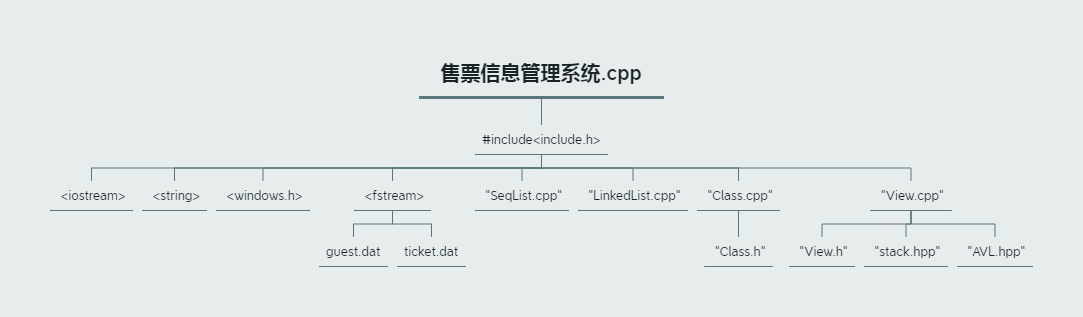
\includegraphics[scale=1,height=5cm,width=0.6\textheight]{1}
\caption{文档结构}
\end{figure}



图片1展示了售票信息管理系统的文档结构,笔者将所有的头文件放入了<include>文件中,将不同的功能模块分成不同的文件,便于代码修改和分工。其中,\textbf{view类}存放了所有的界面,\textbf{class类}存放了用户类和售票信息类。导入了\textbf{fstream}以实现和外部二进制文件\textbf{guest.dat},\textbf{ticket.dat}进行\textbf{IO}操作。

\begin{figure}[htbp]
	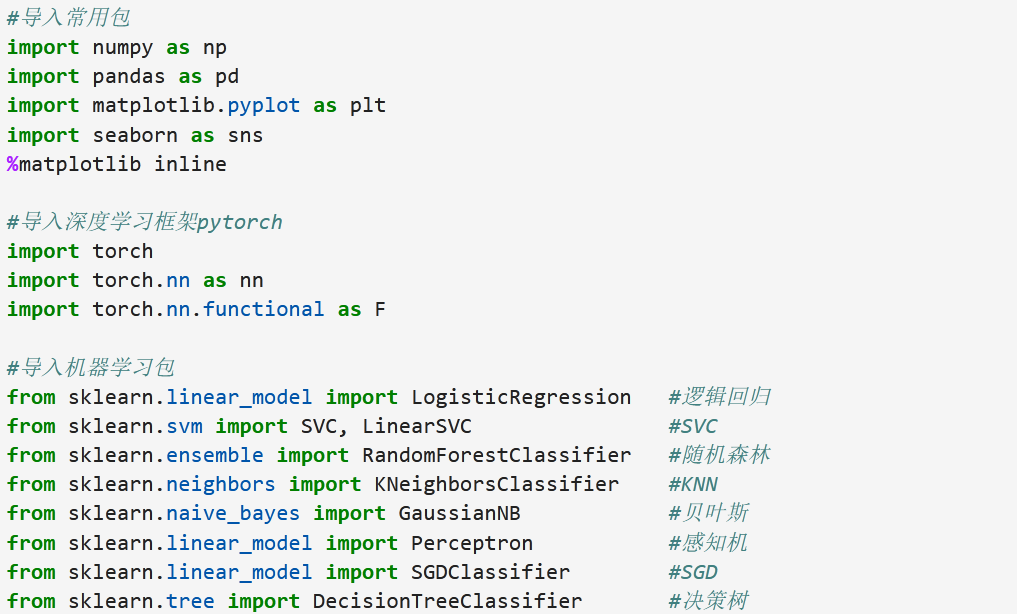
\includegraphics[scale=1,height=7cm,width=0.6\textheight]{2}
	\caption{主函数:通过模块分文件,使主函数简洁易读。}
\end{figure}

图片2中通过\textbf{setconsole}函数简单的对控制台进行了美化。函数定义在头文件windows.h中。\textbf{view}是一个界面对象。



\subsubsection{类}
\begin{figure}[htbp]
	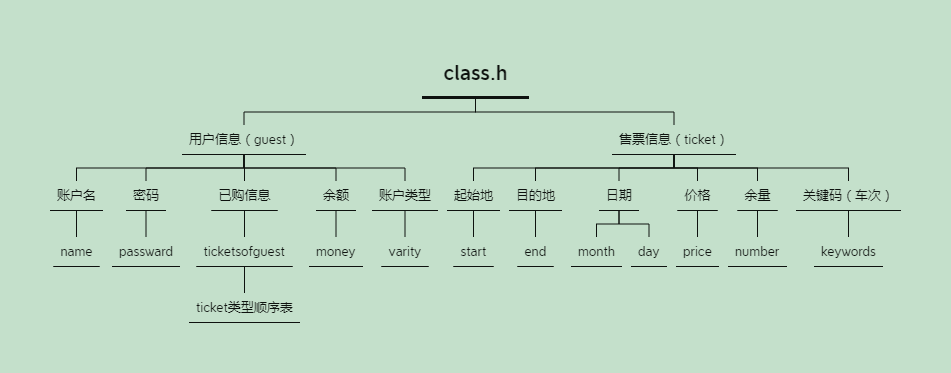
\includegraphics[scale=1,height=5cm,width=0.6\textheight]{3}
	\caption{Class.h结构}
\end{figure}

class.h给出了售票信息系统最重要的两个类:存储用户信息的\textbf{guest类},存储售票信息的\textbf{ticket类}。

ticket类中车次用整数表示,形成了售票信息的唯一关键码,便于后续的\textbf{AVL}树搜索结构的实现。日期包含日和月两部分。
(见附录1)

guest类中\textbf{varity}是一个整数,用于表示当前账户是普通用户还是后台管理员。\textbf{ticketsofguest}是一个顺序表,顺序表中的\textbf{每个元素都是ticket类型的数据},用于存储已经购买车票的信息。(见附录2)




\subsection{文件输入与输出}
售票信息管理系统采用二进制保存信息和读取信息。用户信息保存到guest.dat中,售票信息保存到ticket.dat中。代码见附录4。


\begin{figure}[htbp]
	\subsection{逻辑结构与存储结构}
	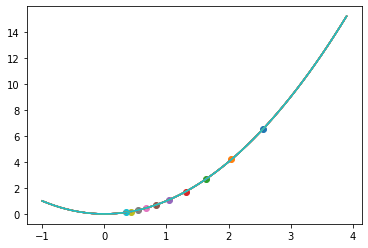
\includegraphics[scale=1,height=6.5cm,width=0.55\textheight]{5}
	\caption{逻辑结构与存储结构}

图4展示了本系统使用的逻辑结构与存储结构,其中guest类嵌套了顺序表,\textbf{顺序表中的每个元素都是ticket类型的对象}。关键码查询时构造了\textbf{AVL}树。
\end{figure}






	\begin{figure}[]
		
		\subsection{运算符重载}
		本系统为了满足查询,输出的要求,对guest,ticket中的运算符进行了重载。
		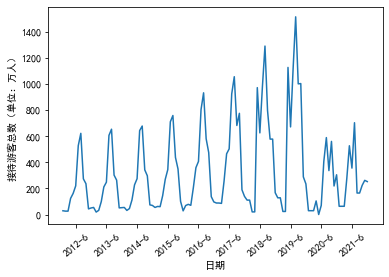
\includegraphics[scale=1,height=5cm,width=0.6\textheight]{6}
		\caption{guest与ticket的重载}
		其中<< 在print函数中使用,直接输出售票信息的信息,代码见附录3.
	\end{figure}
	







\subsection{界面设计}
界面包括主界面,注册和登录界面,注册时分为普通用户和后台管理员,根据账户类型的不同,登录时进入不同的界面。
其中查询使用的是同一个界面,返回时通过判断账户类型返回相应界面,提供三种方式的查询,车次查询构造\textbf{AVL}树进行查询。图6给出所有界面之间的关系。


\begin{figure}[H]
	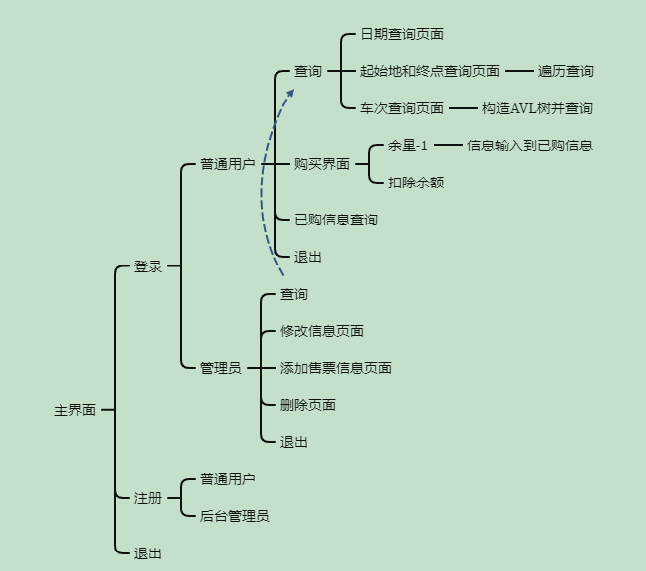
\includegraphics[scale=1,height=12cm,width=0.5\textheight]{4}
	\caption{界面导图}
\end{figure}

 \subsubsection{登录注册界面设计}
 用户在注册时需要选择账户类型,普通用户或者后台管理员,系统界面\textbf{view}中含有一个当前账户的指针,系统会将账户信息记录到指针指向的\textbf{varity},在登录时会根据\textbf{varity}的值进入相应的界面。注意到,普通用户和后台管理员用了同一个查询界面,因此,从查询界面返回普通用户或者后台管理员界面时 ,也会根据该变量的值做出相应的“选择”。
 
 \begin{figure}[H]
 	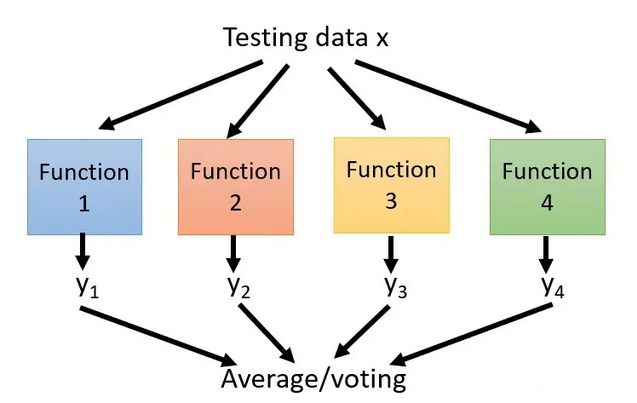
\includegraphics[scale=1,height=6cm,width=0.6\textheight]{7}
 	\caption{注册界面}
 \end{figure}
 
 图7给出了一个注册界面的流程图,其他界面类似,注册界面代码见附录4。类似地,我们做出所有界面。

\subsection{搜索功能的实现}
本系统提供了三种方式的搜索:按日期搜索,按初始地终点搜索,按车次搜索。其中车次搜索使用了\textbf{ticket类AVL树}。
\begin{figure}[H]
	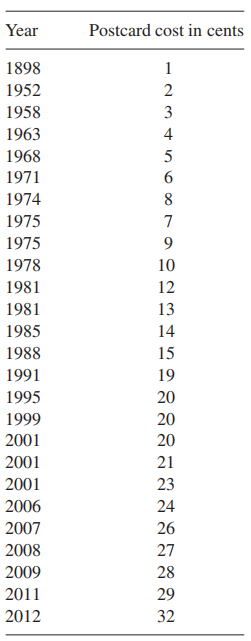
\includegraphics[scale=1,height=5cm,width=0.4\textheight]{8}
	\caption{注册界面}
\end{figure}






\section{系统运行结果及使用说明}
\subsection{系统运行结果}
 通过不断调试与修改,售票信息管理系统实现了售票信息的界面设计与实现,售票信息管理系统包含登录注册功能,并分为\textbf{普通用户}和\textbf{后台管理员}界面,普通用户具有购票,查询,充值,查询历史订单等功能;后台管理员可以添加,修改,删除,查询售票信息。售票信息管理系统关闭时将用户信息与售票信息保存至\textbf{二进制}文件中,打开时读取用户信息和售票信息。
 \begin{figure}[H]
 	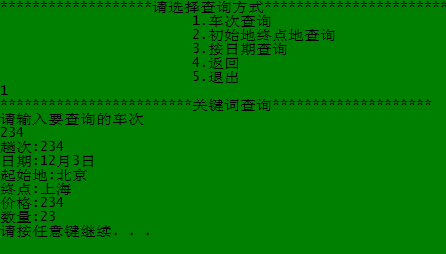
\includegraphics[scale=1,height=6cm,width=0.4\textheight]{9}
 	\caption{查询的一个例子}
 \end{figure}
 



\subsection{使用说明}
1.在使用之前,请先进行\textbf{注册},普通游客没有删除和添加的权利;后台管理员没有购票的权利。\\
2.如果你是普通游客,再购票之前,请先进行\textbf{充值},以保证有充足的余额购票。\\
3.在购票或删除之前请先\textbf{查询}要购买的车次。日期分为月份和号数。\\
4.请不要直接关闭系统,请使用界面菜单进行退出,否则你本次的信息不会保存。





\section{结论与改进}


\subsection{运算符重载重载}
当我们遇到一些复杂结构时候,为了能够对对象进行操作,我们需要对其进行运算符重载。

运算符重载包括类内重载和类外重载,若参数用value表示,目数用number表示,类内重载因为含有this指针$$value=number-1$$,而在类外$$value=number$$
\subsection{模板类产生的类链表}
本售票信息管理系统采用了模板类链表,而这里的T是一个类,因此我们遇到了这样的写法\begin{figure}[H]
	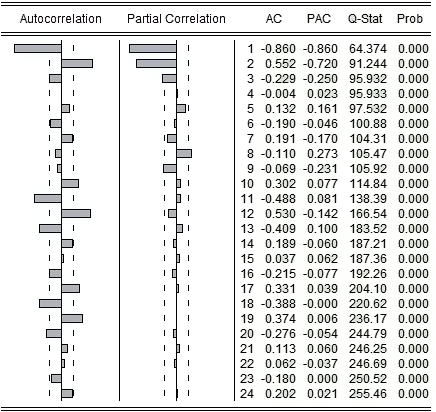
\includegraphics[scale=1,height=1.5cm,width=0.7\textheight]{10}
	\caption{对象的对象}
\end{figure}
其实我们只要把模板T看作是一个整体,当把它单独拿出来的时候,再把它拆分开,对它进行操作。这正是模板类的精髓之处。


	
\subsection{序列化输出类链表}
正是因为类链表中含有类顺序表,导致数据结构变得复杂,因此二进制输入输出不能将guest中的顺序表输出,本系统仅仅将用户信息输出,购票历史没有输出,这正是本系统的缺陷,也是未来的改进方向。

\textbf{序列化 (Serialization)}是将对象的状态信息转换为可以存储或传输的形式的过程。在序列化期间,对象将其当前状态写入到临时或持久性存储区。以后,可以通过从存储区中读取或反序列化对象的状态,重新创建该对象。通过序列化方式将两个链表数据输入到一个文件中是未来的改进方向。














%参考文献
\begin{thebibliography}{9}%宽度9
\bibitem{1}李杨,李雯,胡志鹏,戴琳琳.12306互联网售票系统余票数据一致性保障技术方案研究[J].铁路计算机应用,2021,30(04):11-16.
\bibitem{2} Y.Daniel Liang, Introduction to Programming, 北京:机械工业出版社, 2020.
\bibitem{3} 殷人昆, 数据结构:用面向对象方法与C++语言描述, 北京:清华大学出版社,2007.6
\end{thebibliography}

\newpage
%附录

\section{Appendix}
\begin{lstlisting}[language=c++,caption={ticket类}]
class ticket
{
public:
int keywords;
int month;
int day;
char start[10];
char end[10];
int price;
int number;
public:
bool ifkeywords(int n);
void print();
friend ostream& operator<<(ostream& os, const ticket& c);
};
 \end{lstlisting}
 
 
 
\begin{lstlisting}[language=c++,caption={guest类}]
class guest
{
public:
char name[10];
char passward[15];
int money;
SeqList<ticket> ticketsofguest;
int varity;
public:
void print();
};
 \end{lstlisting}
 
 
 \begin{lstlisting}[language=c++,caption={guest和ticket的运算符重载}]
//*************************************************guest运算符重载***************************************************************
bool operator==(guest a, guest b)
{
return (!strcmp(a.name, b.name) && !strcmp(a.passward, b.passward));
}

bool operator!=(guest& a, guest& b)
{
return strcmp(a.name, b.name) || strcmp(a.passward, b.passward);
}


//*************************************************ticket运算符重载****************************************
void operator&=(ticket& a, ticket& b)
{
a.keywords=b.keywords;
a.month=b.month;
a.day = b.day;
strcpy_s(a.start,b.start);
strcpy_s(a.end,b.end);
a.price=b.price;
a.number = 1;
}

ostream&operator<<(ostream& os, const ticket & c)
{
os << "车次:" << c.keywords << endl;
os << "日期:" << c.month << "月" << c.day << "日" << endl;
os << "出发地:" << c.start << endl;
os << "终点:" << c.end << endl;
os << "价格:" << c.price << endl;
return os;
}
 \end{lstlisting}
 
 \begin{lstlisting}[language=c++,caption={注册界面代码}]
 void View::signinview()
 {
 while(1)
 {
 system("cls");
 cout << "请输入账号" << endl;
 char a[10];
 char b[15];
 char c[15];
 cin >> a;
 cout << "请输入密码" << endl;
 cin >> b;
 cout << "确认密码" << endl;
 cin >> c;
 if (!(strcmp(b,c)))
 {
 cout << "请选择注册类型" << endl;
 cout << "   			1.普通游客" << endl;
 cout << "   			2.后台管理员" << endl;
 int d;
 cin >> d;
 guest current;
 strcpy_s(current.name,a);
 strcpy_s(current.passward, b);
 current.varity = d;
 guests.insert(0,current);
 
 
 system("cls");
 cout << "********************注册成功!************************" << endl;
 cout << "   		1.返回主界面" << endl;
 cout << "   		2.登录" << endl;
 cout << "   		3.退出" << endl;
 cout << "***************************************************" << endl;
 int n;
 cin >> n;
 
 switch (n)
 {
 case 1:MainView(); break;
 case 2:loginview(); break;
 case 3:shutdownview();
 default:signinview();
 }
 
 break;
 }
 else
 {
 system("cls");
 cout << "********************两次输入密码不一致,是否重新注册************************" << endl;
 cout << "   			1.重新注册" << endl;
 cout << "   			2.返回主界面" << endl;
 cout << "   			3.退出" << endl;
 cout << "***************************************************" << endl;
 int n;
 cin >> n;
 
 switch (n)
 {
 case 1:signinview(); break;
 case 2:MainView(); break;
 case 3:shutdownview();
 default:loginview();
 }
 
 }
 }
 }	
 \end{lstlisting}
 
 


\end{document} 